\documentclass[11pt]{article}

\usepackage[letterpaper,margin=1in,footskip=.5in]{geometry}
\usepackage{kpfonts}
\renewcommand{\familydefault}{\sfdefault}
\normalfont 

%Fonts
\usepackage[scaled]{helvet}
\renewcommand\familydefault{\sfdefault} 
\usepackage[T1]{fontenc}

\usepackage{amsmath,fullpage,color,epsfig,bm,wrapfig,harvard,graphicx,epstopdf,float,subfig,amsthm}
\usepackage[    pdftex,    colorlinks,    hyperindex,    plainpages=false,    bookmarksopen,    bookmarksnumbered  ]{hyperref}
\usepackage[bold]{hhtensor}
\usepackage{nicefrac}

\usepackage[colorlinks]{hyperref} 
\hypersetup{ %Sets up hyperref
    %bookmarks=true,         % show bookmarks bar?
    %unicode=false,          % non-Latin characters in Acrobat?s bookmarks
    %pdftoolbar=true,        % show Acrobat?s toolbar?
    %pdfmenubar=true,        % show Acrobat?s menu?
    %pdffitwindow=false,     % window fit to page when opened
    %pdfstartview={FitH},    % fits the width of the page to the window
    pdftitle={Proposal},    % title
    pdfauthor={Jaime Marian},     % author
    colorlinks=true,       % false: boxed links; true: colored links
    linkcolor=red,          % color of internal links
%    linkcolor=black,          % color of internal links
    citecolor=blue,        % color of links to bibliography
    filecolor=magenta,      % color of file links
    urlcolor=cyan           % color of external links
}
\usepackage{cite}
\usepackage{enumitem}
\usepackage{authblk}
\usepackage{multirow}
\usepackage{etoolbox}
\patchcmd{\thebibliography}{\section*{\refname}}{}{}{}
\addtolength{\textwidth}{.25in}
\addtolength{\topmargin}{.1in}
\addtolength{\textheight}{.25in}
\usepackage{tikz}
\usetikzlibrary{arrows,decorations.pathmorphing,backgrounds,positioning,fit,calc,3d,er,trees}
\usepackage{enumitem} %for itemize left margin
\usepackage{overpic}
\usepackage{float}
\usepackage{cases}
\graphicspath{{./Figures/}}

\title{{\Huge\textcolor{red}{Renewable Energy}}}
\author{Nasr Ghoniem\\Distinguished Research Professor\\University of California, Los Angeles (UCLA)\\~ \\\textbf{Course Syllabus}}
\date{\today}

\begin{document}

\maketitle
\tableofcontents
\newpage
\section{Your Instructor}
Professor Ghoniem joined the faculty at UCLA in 1977 as an Assistant Professor after finishing his
Ph.D. in Nuclear Engineering from the University of Wisconsin, Madison. He was promoted to
Associate Professor in 1982, Full Professor in 1986, Senior Professor in 1996, and “Distinguished
Professor” in 2006. Currently, he is a "Distinguished Research Professor" with dual appointments in the departments of Mechanical and Aerospace Engineering, and Materials Science \& Engineering at UCLA. He has wide experience in the development of materials in extreme environments (Nuclear, Mechanical and Aerospace). He is a fellow of the American Nuclear Society, the American Academy of Mechanics, the American Society of Mechanical Engineers, the Japan Society for Promotion of Science, and The Materials Research Society.
\begin{wrapfigure}{r}{.4\textwidth}
	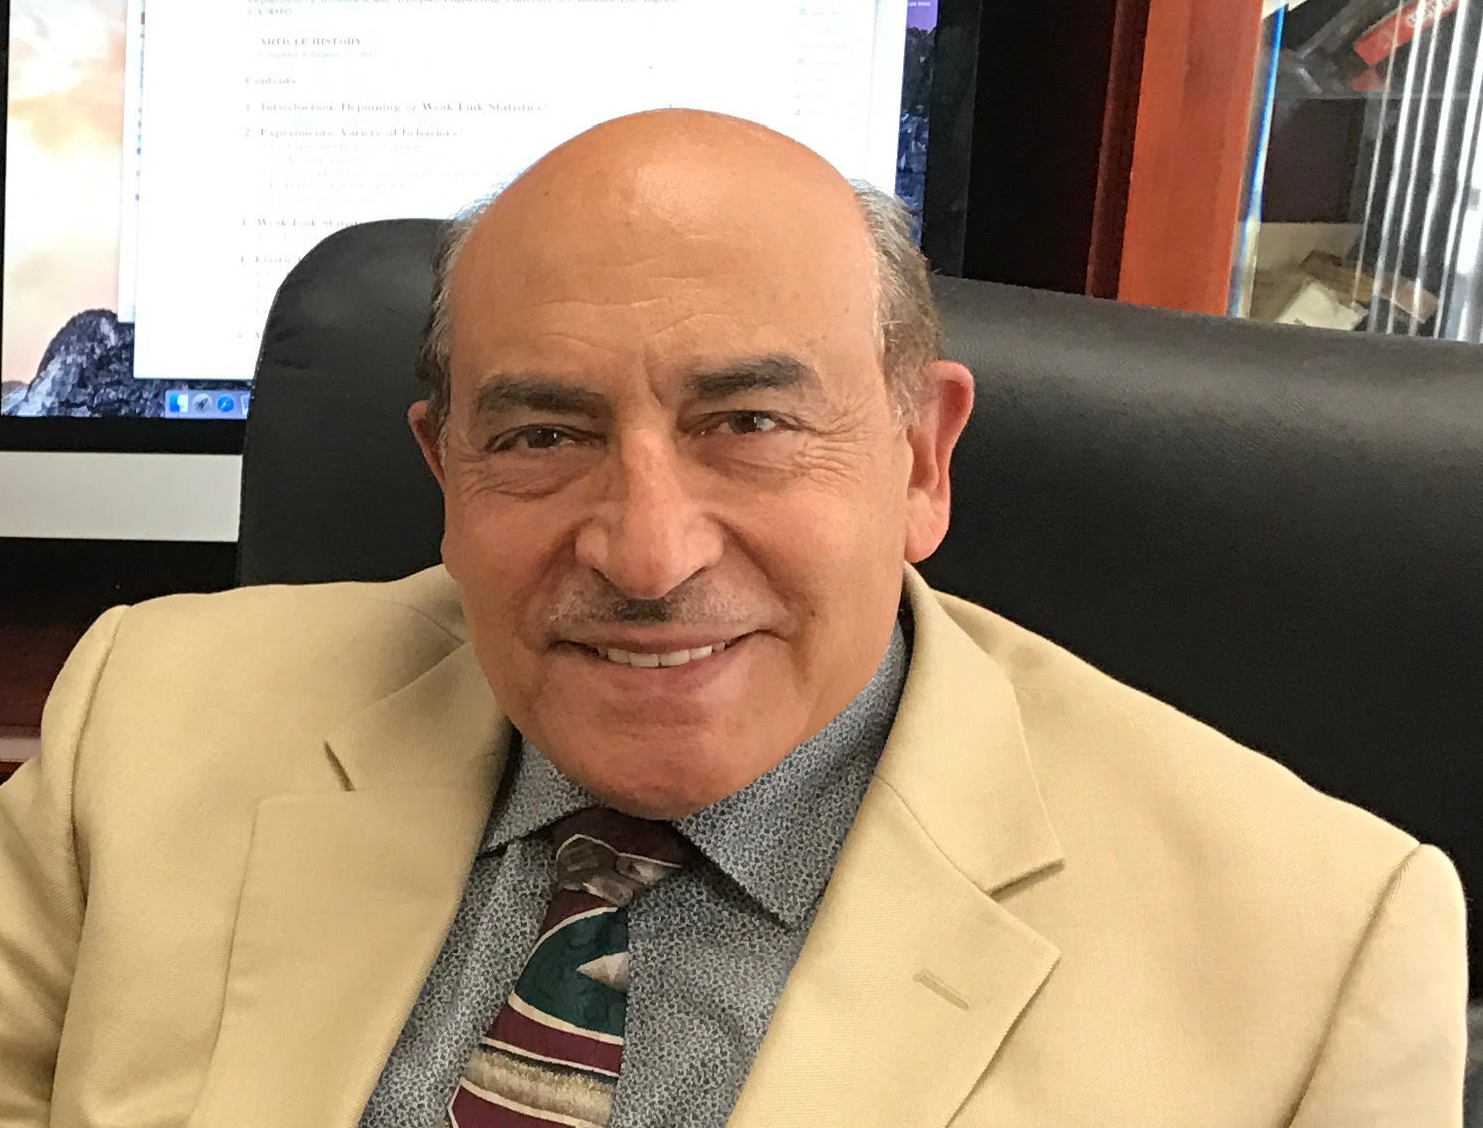
\includegraphics[width=0.4\textwidth]{Nasr-Pic}
\end{wrapfigure}

He was the general chair of the Second International Multiscale Materials Modeling Conference in 2004 and the chair of the 19$^{th}$ International Conference on Fusion Reactor Materials in 2019.  He serves on the editorial boards of several journals, and has published over 350 articles, 10 edited books, and is the co-author of a two-volume book (Oxford Press) on the mechanics and physics of defects, computational materials science, radiation interaction with materials, instabilities and self-organization in non-equilibrium materials (Oxford  Press, 2007, 1100 pages.)  He graduated 41 Ph.D. students and 25 post-doctoral scholars. 16 of his former students and post-docs are currently professors in various universities around the world, and many of his former students are technology leaders in the United States. 
\section{Course Overview and Objectives}
The Renewable Energy course provides introductory-level tutorials on the 
conversion principles and technologies in various clean energy sources, such as solar, wind, hydro, biomass, and geothermal. We examine the issues involved in the thermodynamics, design and operation of three main systems: solar, biomass, and hydro-power during the first four weeks of the class. We also discuss the integration of various clean energy sources and their economics. The second part of the class (last four weeks) will be dedicated to enhancing the research experience of students, where three or more groups will conduct independent research under my supervision. At the completion of this course you will be able to:
\begin{itemize}
    \item Understand the principles of operation of several clean energy technologies.
    \item Analyze the "system" aspects of clean energy technologies.
     \item Realize the technical and economic challenges of each system.
    \item Learn the fundamental principles of thermodynamic energy conversion.
    \item Learn research tools and write a report on the design, operation, integration, or economics of a selected system.
\end{itemize}

Examples of research projects are: design \& operation of solar-thermal power plants; Physics of solar-voltaic systems; Current research and developments in solar photovoltaic materials and systems; design of energy storage systems; material selection in solar, hydro, biomass, wind, or ocean system; design \& operation of wind, ocean, or biomass system; integration \& economics of renewable energy systems. Several research tools will be taught to participating students during the second half of the class. These include: (i) technical writing of reports and papers; (ii) research sources and references; (iii) data representations and graphics.

Students are expected to spend three hours per week with the instructor, and an additional 3-4 hours per week on homework assignments and research projects.
\section{Required Textbook}
\begin{enumerate}
\item Peake, Stephen. \emph{Renewable Energy: Power for a Sustainable Future}, Fourth Edition, 2018, {\bf{Oxford University Press}}, EISBN 978-0-19-253777-5. 
2012.
\item Online lesson content: All other materials are available online through the Neoscholar course website.
\end{enumerate}
\section{Assignments}
A variety of assignments will be given to students to enhance their learning experience and understanding.  These include:
\begin{itemize}
\item \textbf{Discussions}: Each lesson will have discussion questions clearly identified in the lesson content. 
You are to comment on these questions as well as respond to another 
student's comment to earn your full participation grade for this category.
\item \textbf{Homework Assignments}: There will be several homework assignments throughout the course. They 
will cover material from multiple lessons per assignment.
\item \textbf{Quizzes}: Pop Quizzes are expected during lecture hours.  Each quiz is 15 minutes.
\item \textbf{Research Project}: There will be a team project in this course that requires students to work together  on a feasibility study for a renewable energy development project in a location of their choice 
using the technologies and tools presented in this class. More details will be provided several 
weeks into the course. A proposal will be required approximately on the six week of the class.
\item Citation and Reference Style: These will follow the guidelines established in a report template to be provided to students.
\end{itemize}
\newpage

\section{Grading}
	
	\begin{table}[h!]
	    \centering
	    \begin{tabular}{|l|l|}
	         	\hline\hline
	Grade Category	& Percent of the Grade		\\
		\hline\hline  
		Homework	& 15\%	\\
		Discussions	& 15\%	\\
		Quizzes & 10\%\\
		Research Project	& 60\%	\\
		\hline\hline
	    \end{tabular}
	    \caption{Grading Scheme}
	    \label{tab:grades1}
	\end{table}
	
	\begin{table}[h!]
	    \centering
	    \begin{tabular}{|l|l|}
	         	\hline\hline
	Letter Grade	& Percentage		\\
		\hline\hline  
		A+	& $>$95\%	\\
		A	& 90-95\%	\\
		A-	& 85-90\%	\\
		B+	& 80-85\%	\\
		B & 75-80\%\\
		B-& 70-75\%\\
		C&$<70\%$\\
		\hline\hline
	    \end{tabular}
	    \caption{Letter grade percentages}
	    \label{tab:grades2}
	\end{table}
	
	\newpage
	\section{Course Schedule}
	\subsection*{Week 1}
	\begin{itemize}
	    \item Class orientation.
	    \item Global energy use.
	    \item Fossil fuels and climate change.
	    \item Overview of renewable energy sources.
	    \item Reading Assignment: Chapter 1 - Introducing Renewable Energy.
	 \item Laws of thermodynamics.
	    \item Fuels \& combustion.
	\end{itemize}
	\subsection*{Week 2}
	\begin{itemize}
	 \item Heat engines.
	    \item Heat pumps.
	    \item Reading Assignment: Chapter 2 - Thermodynamics, heat engines, and heat pumps.
		 \item Solar Thermal Energy
	    \item Availability of solar energy
	    \item Low-temperature applications.
	    \item Active versus passive heating.
	    \item Electricity generation.
	    \item Economics \& environmental impact.
	    \item Reading Assignment: Chapter 3 - Solar-Thermal Energy.
	    \end{itemize}
	\subsection*{Week 3}
	\begin{itemize}
\item Solar photovoltaics basic principles
	    \item Polycrystalline and thin film photovolatics.
	    \item PV grid-connected systems \& integration.
	    \item Environmental impact \& economics.
	    \item Reading Assignment: Chapter 4 - Solar Photovoltaics.
	\end{itemize}
		\subsection*{Week 4}
	\begin{itemize}
	  \item Bioenergy sources
	    \item Combustion of solid biomass.
	    \item Fuel production (gaseous and liquid).
	    \item Environmental impact \& economics.
	    \item Reading Assignment: Chapter 5 - Bioenergy.
	\end{itemize}
	\subsection*{Week 5}
	\begin{itemize}
	  \item History of water power.
	    \item Hydro resources.
	    \item Types of hydroelectric plants.
	    \item Turbines.
	    \item Integration 
	    \item Environmental impact \& economics.
	    \item Reading Assignment: Chapter 6- Hydroelectricity.
	    \item Project orientation and team assignments.
	\end{itemize}
	\subsection*{Week 6}
	Discussion and selection of research projects: 
	\begin{enumerate}
	    \item Design \& operation of solar-thermal or solar-voltaic systems; 
	    \item Design of energy storage systems; 
	    \item Material selection in solar, hydro, biomass, wind, or ocean system; 
	    \item Design \& operation of wind, wave, geothermal, or biomass system; 
	    \item Issues for integration \& economics of renewable energy systems.
	    and references.
	\end{enumerate} 
\subsection*{Week 7}
\begin{itemize}
    \item Technical writing tutorial.
    \item Research project preliminary report outline.
    \item Discussion of research resources and references.
    \item Team interactions and project guidance.
   \item Guided discussions on team projects.
\end{itemize}
\subsection*{Week 8}
\begin{itemize}
    \item Team project presentations.
    \item Research reports discussions.
    \item Research reports turned in and graded.
\end{itemize}
\newpage
\section{Project Description}

Renewable energy sources are important in two respects: (1) they can be sustainable for long periods; and (2) they are carbon-free or have low-carbon emissions.  Nevertheless, many technologies are still emerging and are in the process of intense development. There are many constraints that affect the rapid development and introduction of renewable energy sources. These are mainly economic, but some limitations are also related to the society and its acceptance of such technologies. The world will need many
professionals with a deep knowledge of renewable energy technologies.  Key to such expertise is understanding the 
underlying physical and technological principles, their economics and market needs, their environmental impact, and the likelihood that they can be integrated within existing energy grids, especially within the concept of "smart grids."

In this project, a team of students will develop a concept report that addresses one particular renewable energy source, and make a presentation of their findings at the end of the course.  The guidelines for the project, associated report, and group presentation are:
\begin{enumerate}
    \item Select a renewable energy source, and develop a research plan.  The energy source may be from the following list.
    \begin{itemize}
        \item Heat pumps.
        \item Rooftop solar thermal water heater.
        \item Domestic solar heating systems.
        \item Active solar heating and design of solar collectors.
        \item Passive solar heating of residential and commercial building. 
        \item Solar thermal engines, power plants and electricity generation.
        \item Solar photovoltaics: physics \& technology.
        \item Large, grid-connected Solar photovoltaic power plants.
        \item Biomass resources.
        \item Bioenergy conversion technologies.
        \item Hydroelectric power plants.
        \item Tidal energy technologies: barrages, lagoons, \& streams.
        \item Electric power from wind energy.
        \item Wave energy technology.
        \item Deep geothermal energy.
    \end{itemize}
    \item Make an outline for your project and final report.  Your outline may include some of the following:
    \begin{itemize}
        \item Introduction
        \item History
        \item Physics \& technology principles
        \item Description of a typical system, engine, or power plant.
        \item Integration in energy grid.
        \item Environmental impact
        \item Economics
        \item Future developments
        \item Conclusions
        \item References
        \item Appendices
    \end{itemize}
    \item Perform research on the topic in consultation with the Teaching Assistant and your team members.
    \item Divide up the report writing tasks amongst team members.
    \item Prepare the project report as a collaborative effort with participation of all team members. The report is expected to be between 15-20 pages long.
    \item prepare a power point presentation to the class, to be given the last day of instruction.
    \item A few short lectures will continue throughout week 7 of the class to cover materials from earlier weeks.
\end{enumerate}
\end{document}
